\documentclass{article}
\usepackage{graphicx}
\usepackage{authblk}
\usepackage{listings}
\usepackage{xcolor}
\usepackage[a4paper,
            bindingoffset=0.2in,
            left=0.5in,
            right=0.5in,
            top=0.75in,
            bottom=0.75in,
            footskip=.25in]{geometry}

\definecolor{mGreen}{rgb}{0,0.6,0}
\definecolor{mGray}{rgb}{0.5,0.5,0.5}
\definecolor{mPurple}{rgb}{0.58,0,0.82}
\definecolor{backgroundColour}{rgb}{0.95,0.95,0.92}

\lstdefinestyle{CStyle}{
    backgroundcolor=\color{backgroundColour},   
    commentstyle=\color{mGreen},
    keywordstyle=\color{magenta},
    numberstyle=\tiny\color{mGray},
    stringstyle=\color{mPurple},
    basicstyle=\footnotesize,
    breakatwhitespace=false,         
    breaklines=true,                 
    captionpos=b,                    
    keepspaces=true,                 
    numbers=left,                    
    numbersep=5pt,                  
    showspaces=false,                
    showstringspaces=false,
    showtabs=false,                  
    tabsize=2,
    language=C
}


\title{Assignment \#1 - Standard I/O, Math, and if/else}
\author{Cody Raposa}
\affil{ELEC2850 Microcontrollers Using C Programming}

\begin{document}
\maketitle
\begin{flushleft}
	\section{Question 1}
	\subsection{}
	Answer is b. \{\}
	\subsection{}
	Answer is c.
	\subsection{}
	Answer is b. No.
	\subsection{}
	Answer is b. A semicolon ;
	\subsection{}
	Answer is c. The Screen.
	\newpage
	\section{Q2 Problem Statement}
	Create a program that takes a users two coordinates, formatted by x1,y1 and x2,y2, and calculates the distance between the two points. Then display that distance to the user.
	%\section{Assumptions}
	\section{Algorithm}
	\begin{figure}[!h]
		\begin{centering}
			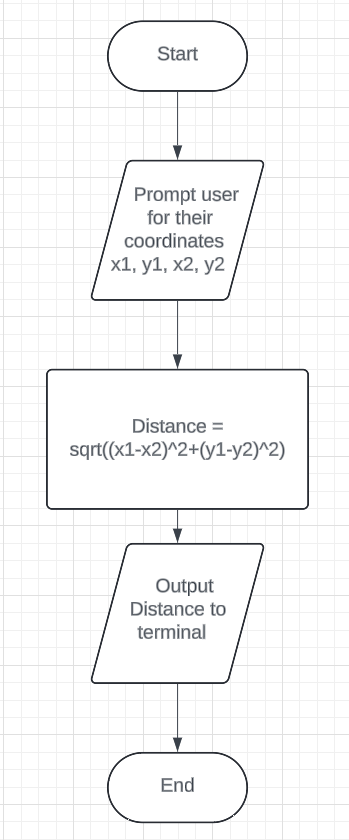
\includegraphics[scale=0.45]{Q2flowchart.png}
			\caption{Flowchart for Question 2}
		\end{centering}
	\end{figure}
	\section{Output}
	\begin{figure}[!h]
		\begin{centering}
			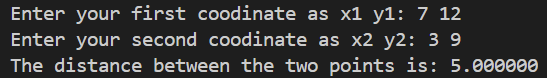
\includegraphics[width=\linewidth]{Q2Output.png}
			\caption{Output for Question 2}
		\end{centering}
	\end{figure}
	\section{Code}
	\lstinputlisting[style=CStyle]{Q2.c}
	\newpage
	\section{Q3 Problem Statement}
	Create a program that takes a users two numbers, and calculates a pythagorean triple from the two numbers. If the first number entered is smaller than the second, prompt the user to switch the two and retry.
	\section{Algorithm}
	\begin{figure}[!h]
		\begin{centering}
			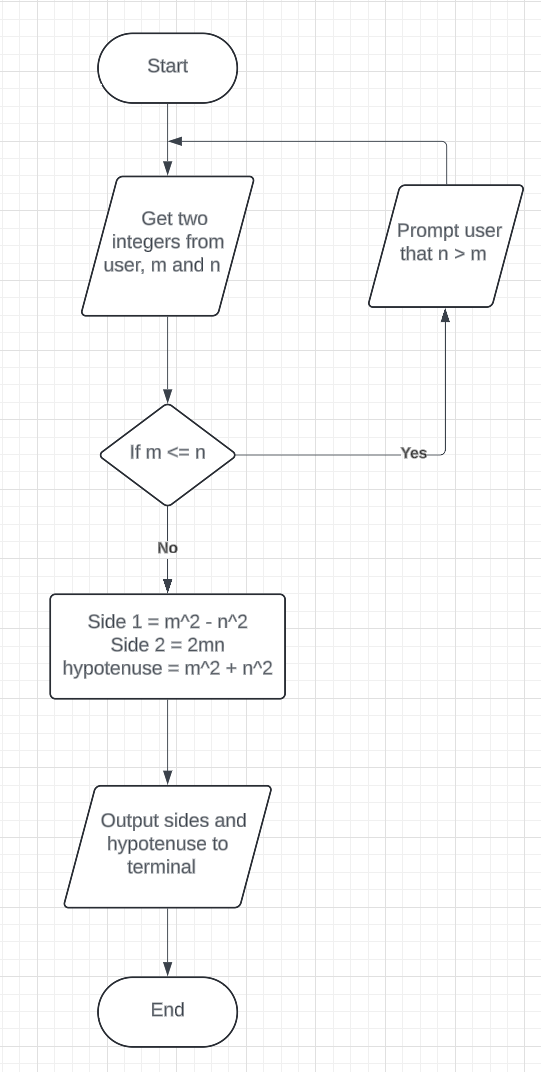
\includegraphics[scale=0.45]{Q3flowchart.png}
			\caption{Flowchart for Question 3}
		\end{centering}
	\end{figure}
	\section{Output}
	\begin{figure}[!h]
		\begin{centering}
			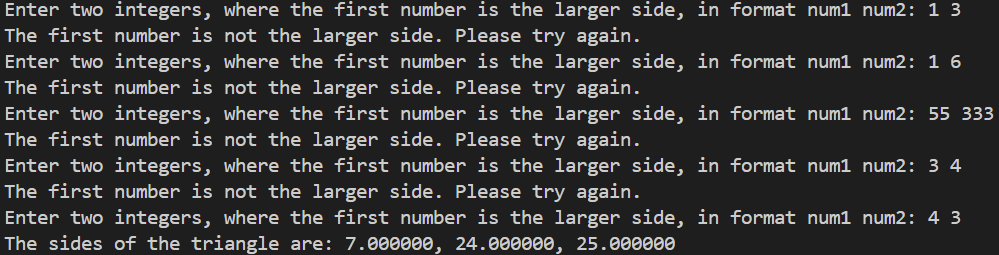
\includegraphics[width=\linewidth]{Q3Output.png}
			\caption{Valid and invalid inputs for Question 3}
		\end{centering}
	\end{figure}
	\section{Code}
	\lstinputlisting[style=CStyle]{Q3.c}
\end{flushleft}
\end{document}